\subsection{Brisanje naloga klijenta}

Ukoliko klijent na stranici ažuriranja profila (slika \ref{fig:AccountSettings}) izabere opciju \textit{Delete account}, pojavljuje se stranica brisanja naloga klijenta (slika \ref{fig:DeleteAccount}). Ova stranica upozorava klijenta da će svi njegovi podaci biti izgubljeni, kao i da će mu sva dugovanja biti automatski naplaćena. Traži se od klijenta da unese svoju šifru kako bi potvrdio brisanje naloga. Klijent može i odustati od brisanja naloga klikom na dugme \textit{Cancel}.
\begin{figure}[H]
	\begin{center}
		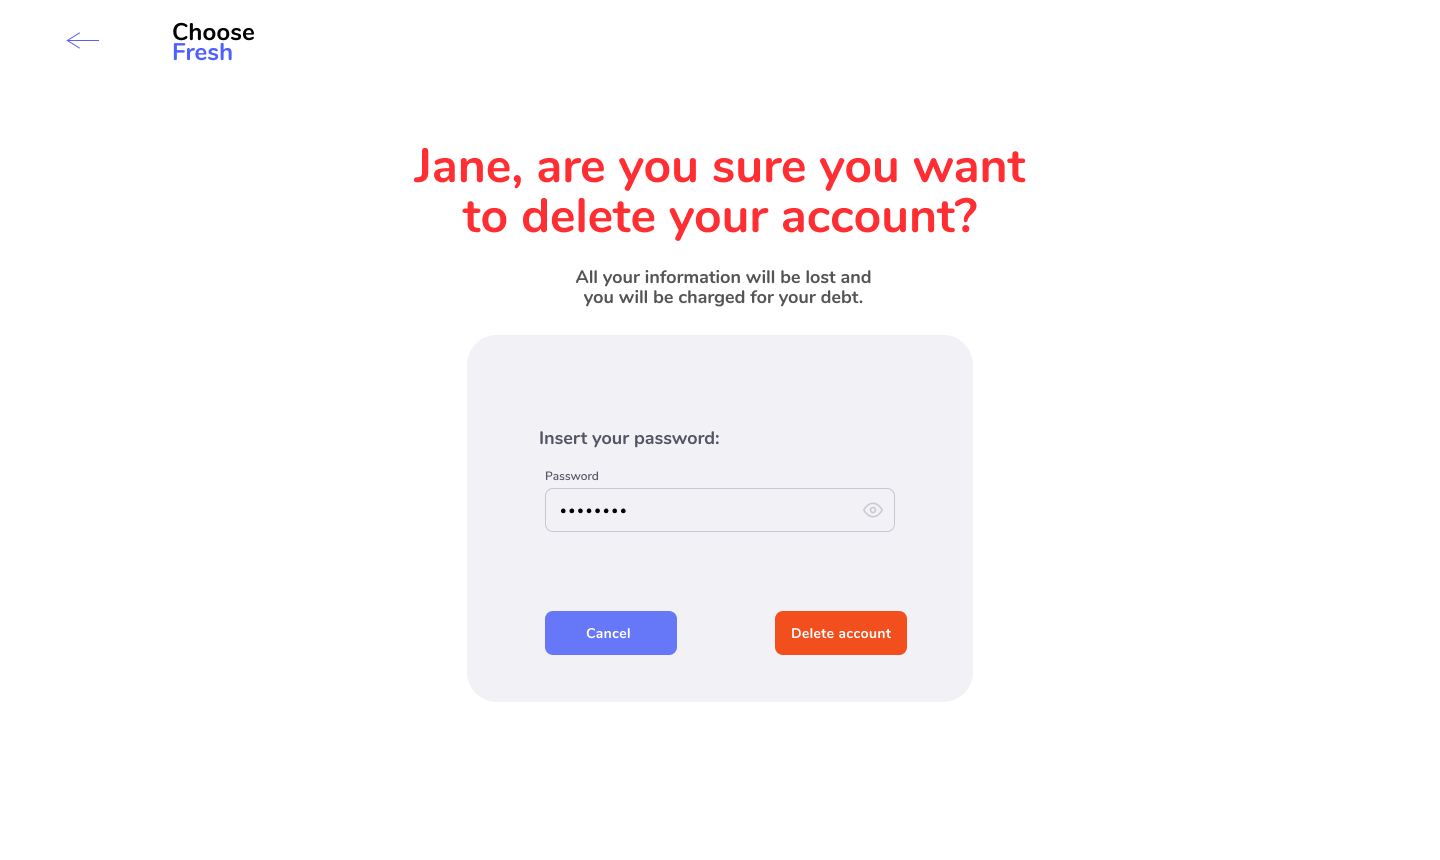
\includegraphics[width=\textwidth]{UI/DeleteAccount.png}
    		\caption{Stranica brisanja naloga klijenta}
    \label{fig:DeleteAccount}
    \end{center}
\end{figure}

Ako je klijent uneo ispravnu šifru i potvrdio opciju za brisanje naloga, pojavljuje se stranica koja obaveštava klijenta da je uspešno obrisao svoj nalog (slika \ref{fig:DeleteAccountSuccessful})

\begin{figure}[H]
	\begin{center}
		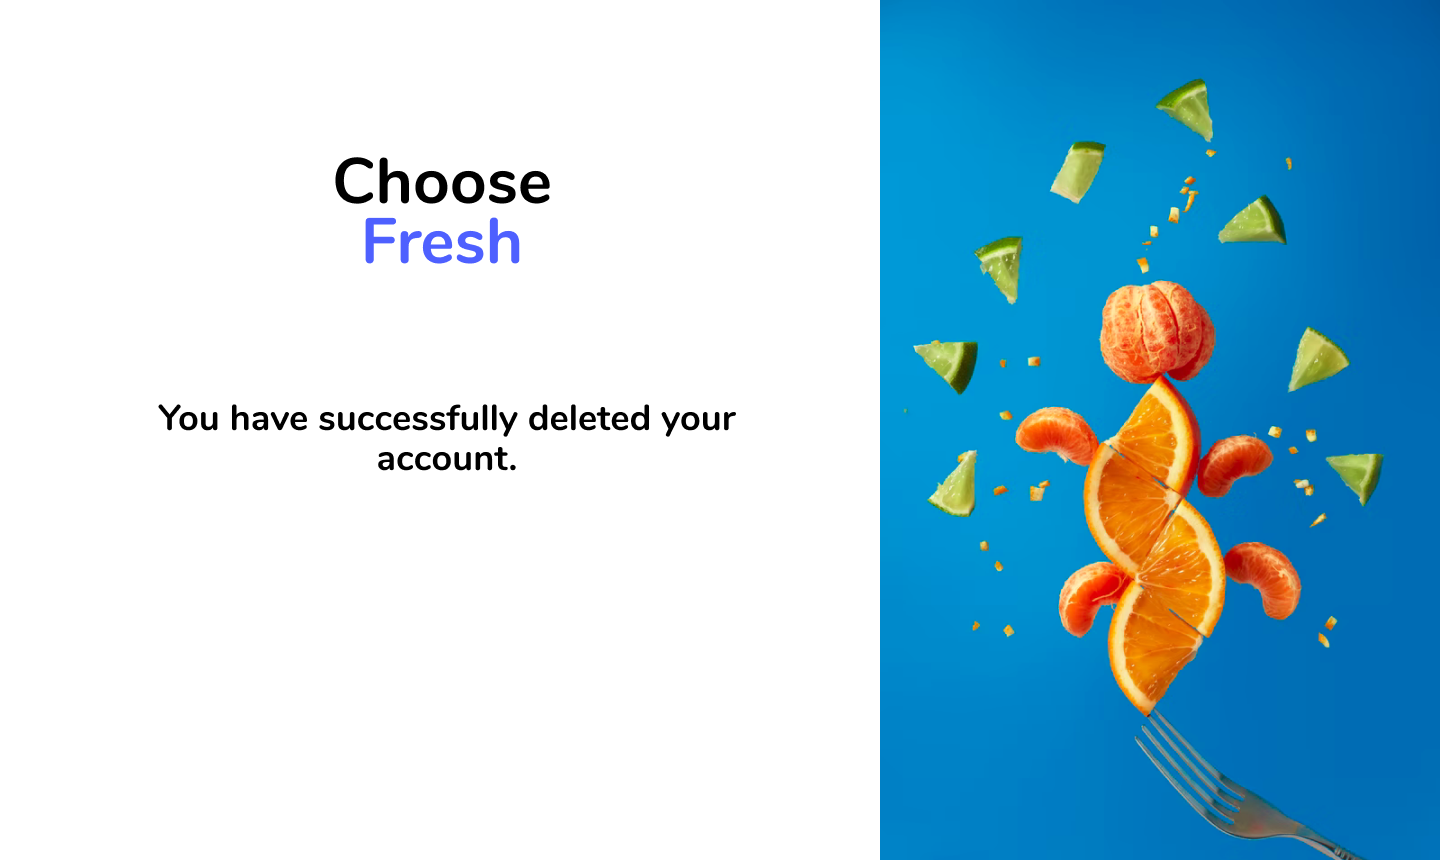
\includegraphics[width=\textwidth]{UI/DeleteAccountSuccessful.png}
    		\caption{Stranica uspešno obrisanog naloga klijenta}
    \label{fig:DeleteAccountSuccessful}
    \end{center}
\end{figure}